\mode*
\part{Processes and Threads}
\lecture{Process}{proc}

\section{Virtual Memory}
\label{sec:virtual-memory}

\begin{frame}{Programs}
A program is a file sitting in your hard disk. Two forms:
\begin{itemize}
\item Source code, e.g. \texttt{hello.c}, human readable
\item Executable code, e.g. \texttt{a.out}, machine readable
  \begin{description}
  \item[Binary format identification] Usually ELF
  \item[Machine-language instructions] Program algorithm
  \item[Entry-point address] Where to find \texttt{main()}?
  \item[Data] Initialized variables
  \item[Symbol and relocation tables] Address of variables, functions...
  \item[Shared-library] Where to find \texttt{printf()}?
  \item[More] ...
  \end{description}
\end{itemize}
\end{frame}

\begin{frame}{Process}
  \begin{description}
  \item[A process] is an instance of a program in execution
  \end{description}
  \begin{minipage}{.65\linewidth}
    \begin{block}{\mbox{Processes are like human beings:}}
        \begin{itemize}
        \item[\Symbol{➠}] they are generated
        \item[\Symbol{➠}] they have a life
        \item[\Symbol{➠}] they optionally generate one or more child processes, and
        \item[\Symbol{➠}] eventually they die
        \end{itemize}
        A small difference:
        \begin{itemize}
        \item sex is not really common among processes
        \item each process has just one parent
        \end{itemize}
      \end{block}
  \end{minipage}\quad
  \begin{minipage}{.3\linewidth}
    \begin{center}
      \mode<beamer>{ 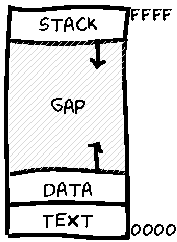
\includegraphics[width=\textwidth]{mos-figs-1-20} }%
      \mode<article>{ 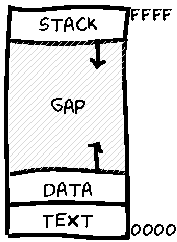
\includegraphics[width=.5\textwidth]{mos-figs-1-20} }
    \end{center}
  \end{minipage}
\end{frame}

\begin{frame}{Problem With Real Mode}
  \begin{center}
    \mode<beamer>{ \includegraphics[width=.7\textwidth]{mm-relocation} }%
    \mode<article>{ \includegraphics[width=.5\textwidth]{mm-relocation} }
  \end{center}
\end{frame}

\begin{frame}{Protected mode}
  We need
  \begin{itemize}
  \item Protect the OS from access by user programs
  \item Protect user programs from one another
  \end{itemize}
  \begin{description}
  \item[Protected mode] is an operational mode of x86-compatible CPU.
    \begin{itemize}
    \item The purpose is to protect everyone else (including the OS) from your program.
    \end{itemize}
  \end{description}
\end{frame}

\begin{frame}{Memory Protection}{Logical Address Space}
  \begin{description}
  \item[Base register] holds the smallest legal physical memory address
  \item[Limit register] contains the size of the range
  \end{description}
  \begin{varwidth}{.48\textwidth}
    \begin{center}
      \mode<beamer>{ 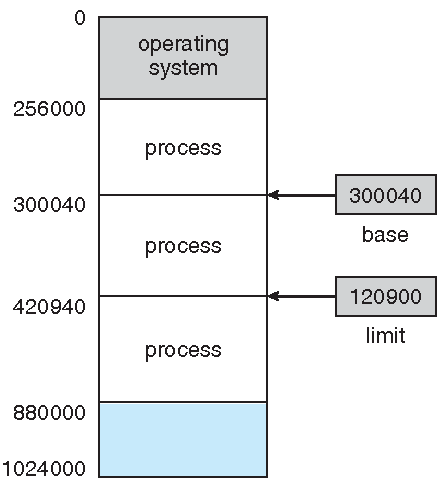
\includegraphics[width=\textwidth]{osc-8-5} }%
      \mode<article>{ 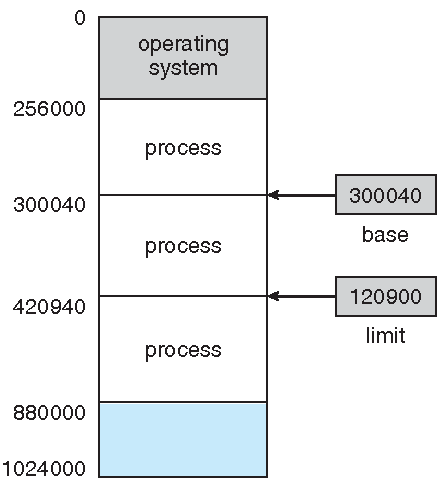
\includegraphics[width=.7\textwidth]{osc-8-5} }
    \end{center}
  \end{varwidth}\hfill
  \begin{varwidth}{.45\textwidth}
    A pair of \texttt{base} and \texttt{limit} registers define the logical address space
    \begin{center}
      \cfbox{violet}{\texttt{JMP 28}}
    \end{center}
    \begin{center}
      {\rotatebox{270}{\huge \Symbol{➠}}}
    \end{center}
    \begin{center}
      \cfbox{violet}{\texttt{JMP 300068}}
    \end{center}
  \end{varwidth}
\end{frame}

\begin{frame}{Memory Protection}{Base and limit registers}
  \begin{center}
    \mode<beamer>{ 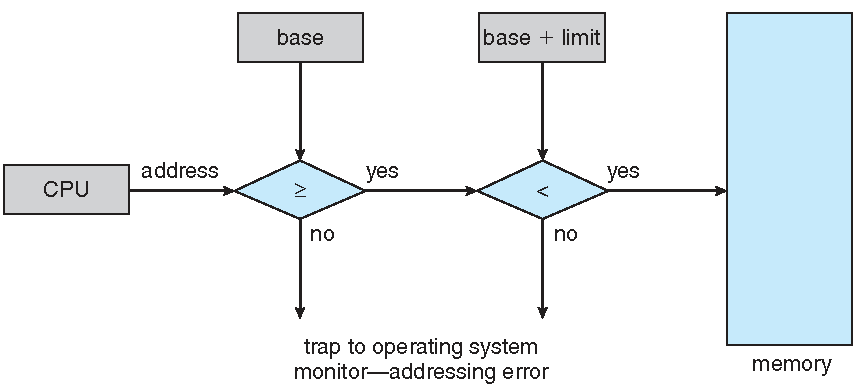
\includegraphics[width=\textwidth]{mm-protection} }%
    \mode<article>{ 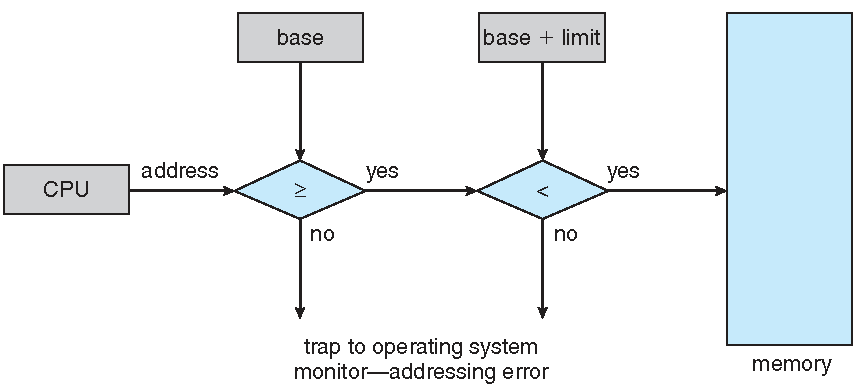
\includegraphics[width=.7\textwidth]{mm-protection} }
  \end{center}
\end{frame}

\begin{frame}{UNIX View of a Process' Memory}
  \begin{varwidth}{.48\textwidth}
    \begin{center}
      \mode<beamer>{ \includegraphics[width=\textwidth]{mm-process} }%
      \mode<article>{ \includegraphics[width=.7\textwidth]{mm-process} }
    \end{center}
  \end{varwidth}\hfill
  \begin{varwidth}{.48\textwidth}
    \begin{itemize}
    \item[text:] program code
    \item[data:] initialized global and static data
    \item[bss:] uninitialized global and static data
    \item[heap:] dynamically allocated with \texttt{malloc, new}
    \item[stack:] local variables
    \end{itemize}
  \end{varwidth}
\end{frame}

\begin{frame}{Stack vs. Heap}
  \begin{center}
    \begin{tabular}{ll}\toprule
      \textbf{Stack}           &\textbf{Heap}\\\midrule
      compile-time allocation &run-time allocation\\
      auto clean-up           &you clean-up\\
      inflexible              &flexible\\
      smaller                 &bigger\\
      quicker                 &slower\\\bottomrule
    \end{tabular}
  \end{center}
  \begin{block}{How large is the ...}
    \begin{description}
    \item[stack:] \texttt{ulimit -s}
    \item[heap:] could be as large as your virtual memory
    \item[text|data|bss:] \texttt{size a.out}
    \end{description}
  \end{block}
\end{frame}

\begin{frame}{Multi-step Processing of a User Program}{When is space
    allocated?}
  \begin{minipage}{.4\textwidth}
    \begin{center}
      \mode<beamer>{ 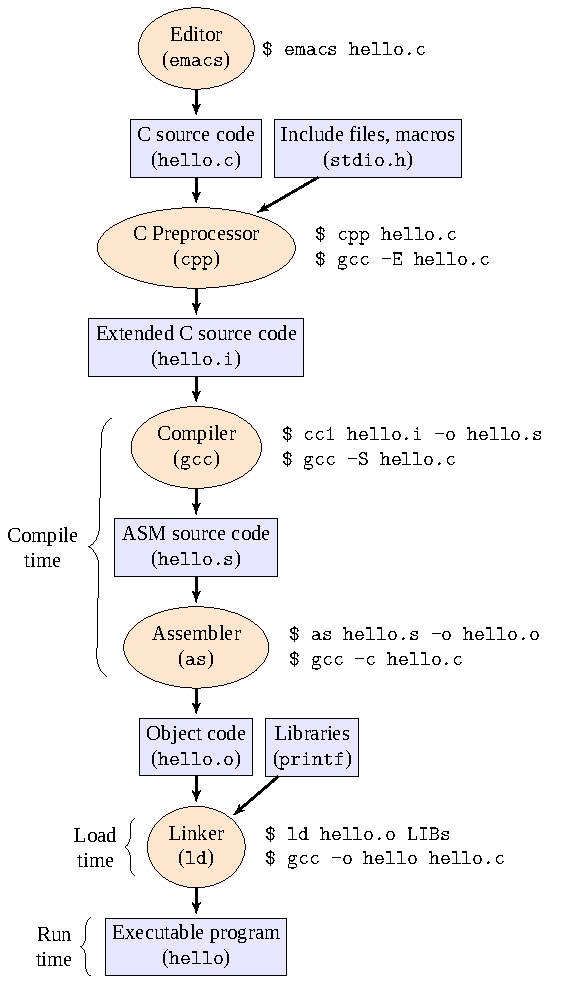
\includegraphics[width=\textwidth]{tool-chain-mm} }%osc-8-7
      \mode<article>{ 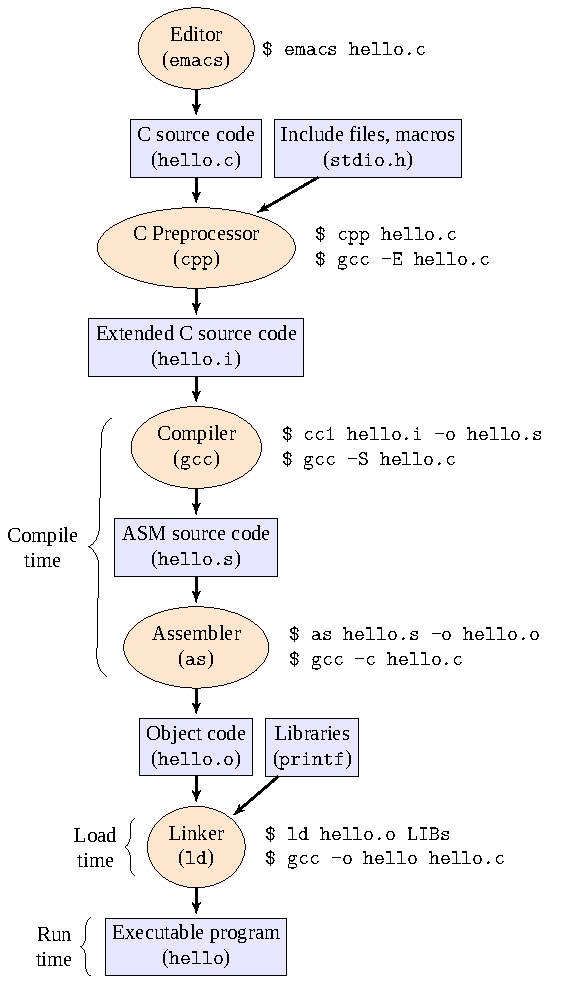
\includegraphics[width=.9\textwidth]{tool-chain-mm} }
    \end{center}
    \label{reg}
  \end{minipage}
  \begin{minipage}{.55\textwidth}
    \begin{small}
      \begin{description}
      \item[Static:] before program start running
        \begin{itemize}
        \item Compile time
        \item Load time
        \end{itemize}
      \item[Dynamic:] as program runs
        \begin{itemize}
        \item Execution time
        \end{itemize}
      \end{description}
    \end{small}
  \end{minipage}
\end{frame}

\begin{description}
\item[Compiler] The name "compiler" is primarily used for programs that translate source
  code from a high-level programming language to a lower level language (e.g., assembly
  language or machine code)\citetitle{wiki:compiler}.
\item[Assembler] An assembler creates object code by translating assembly instruction
  mnemonics into opcodes, and by resolving symbolic names for memory locations and other
  entities\citetitle{wiki:assembler}.
\item[Linker] Computer programs typically comprise several parts or modules; all these
  parts/modules need not be contained within a single object file, and in such case refer
  to each other by means of symbols\citetitle{wiki:linker}.

  When a program comprises multiple object files, the linker combines these files into a
  unified executable program, resolving the symbols as it goes along.

  Linkers can take objects from a collection called a library. Some linkers do not include
  the whole library in the output; they only include its symbols that are referenced from
  other object files or libraries. Libraries exist for diverse purposes, and one or more
  system libraries are usually linked in by default.

  The linker also takes care of arranging the objects in a program's address space. This
  may involve relocating code that assumes a specific base address to another base. Since
  a compiler seldom knows where an object will reside, it often assumes a fixed base
  location (for example,zero).
\item[Loader] An assembler creates object code by translating assembly instruction
  mnemonics into opcodes, and by resolving symbolic names for memory locations and other
  entities. ... Loading a program involves reading the contents of executable file, the
  file containing the program text, into memory, and then carrying out other required
  preparatory tasks to prepare the executable for running. Once loading is complete, the
  operating system starts the program by passing control to the loaded program
  code\citetitle{wiki:loader}
\item[Dynamic linker] A dynamic linker is the part of an operating system (OS) that loads
  (copies from persistent storage to RAM) and links (fills jump tables and relocates
  pointers) the shared libraries needed by an executable at run time, that is, when it is
  executed. The specific operating system and executable format determine how the dynamic
  linker functions and how it is implemented. Linking is often referred to as a process
  that is performed at compile time of the executable while a dynamic linker is in
  actuality a special loader that loads external shared libraries into a running process
  and then binds those shared libraries dynamically to the running process. The specifics
  of how a dynamic linker functions is operating-system
  dependent\citetitle{wiki:dynamic-linker}
\end{description}

Linkers and Loaders allow programs to be built from modules rather than as one big
monolith.

See also:
\begin{itemize}
\item \citetitle[Chap.~7, \emph{Linking}]{Bryant2010computersystems}.
\item COMPILER, ASSEMBLER, LINKER AND LOADER: A BRIEF
  STORY\footnote{\url{http://www.tenouk.com/ModuleW.html}}.
\item Linkers and Loaders\footnote{\url{http://www.iecc.com/linker/}}.
\item \citetitle[\emph{Links and loaders}]{levine2000linkers}.
\item Linux Journal: Linkers and
  Loaders\footnote{\url{http://www.linuxjournal.com/article/6463}}. Discussing how
  compilers, links and loaders work and the benefits of shared libraries.
\end{itemize}

\begin{frame}{Address Binding}{Who assigns memory to segments?}
  \begin{block}{Static-binding: before a program starts running}
    \begin{description}
    \item[Compile time:] \alert{Compiler} and \alert{assembler} generate an object file for
      each source file
    \item[Load time:] \hfill
      \begin{itemize}
      \item \alert{Linker} combines all the object files into a single executable object
        file
      \item \alert{Loader} (part of OS) loads an executable object file into
        memory at location(s) determined by the OS
        \begin{itemize}
        \item[-] invoked via the \texttt{execve} system call
        \end{itemize}
      \end{itemize}
    \end{description}
  \end{block}
  \begin{block}{Dynamic-binding: as program runs}
    \begin{itemize}
    \item Execution time:
      \begin{itemize}
      \item uses \texttt{new} and \texttt{malloc} to dynamically allocate memory
      \item gets space on stack during function calls
      \end{itemize}
    \end{itemize}
  \end{block}
\end{frame}

\begin{itemize}
\item Address binding has nothing to do with physical memory (RAM). It determines the
  addresses of objects in the address space (virtual memory) of a process.
\end{itemize}

\begin{frame}{Virtual Memory}{Logical memory can be much larger than physical memory}
  \begin{varwidth}{.48\textwidth}
    \begin{center}
      \mode<beamer>{ 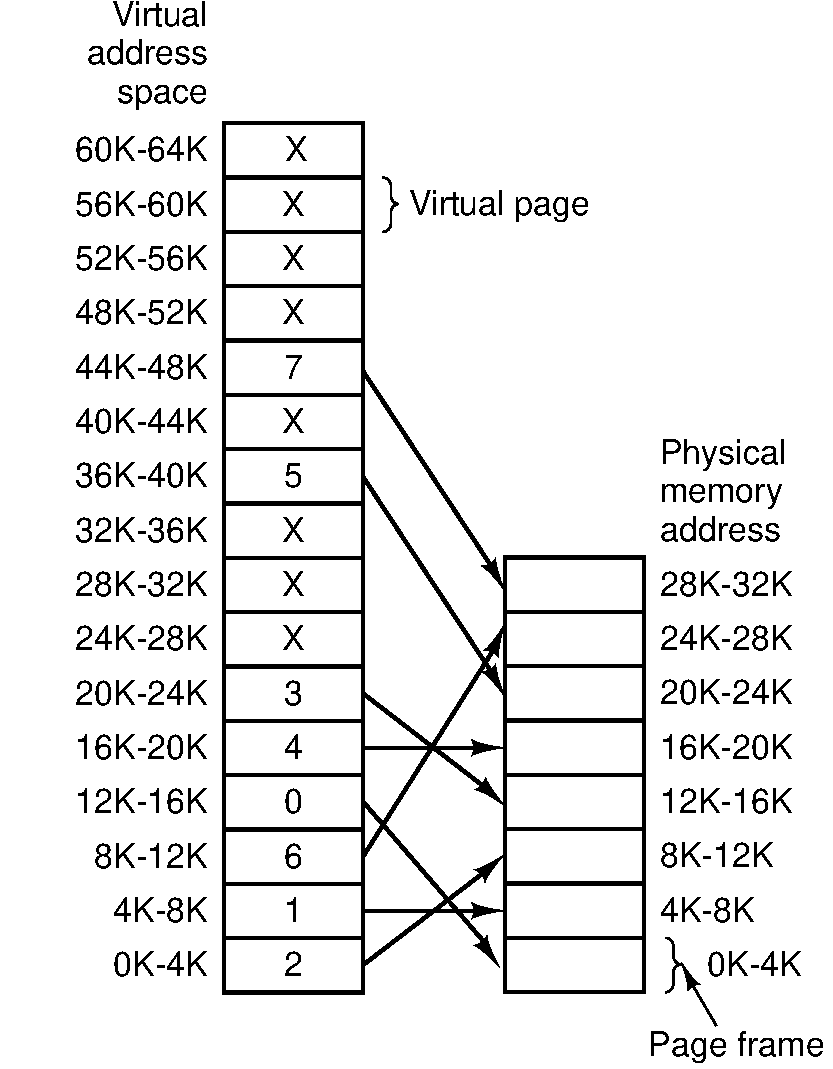
\includegraphics[width=\textwidth]{mos-figs-4-10} }%
      \mode<article>{ 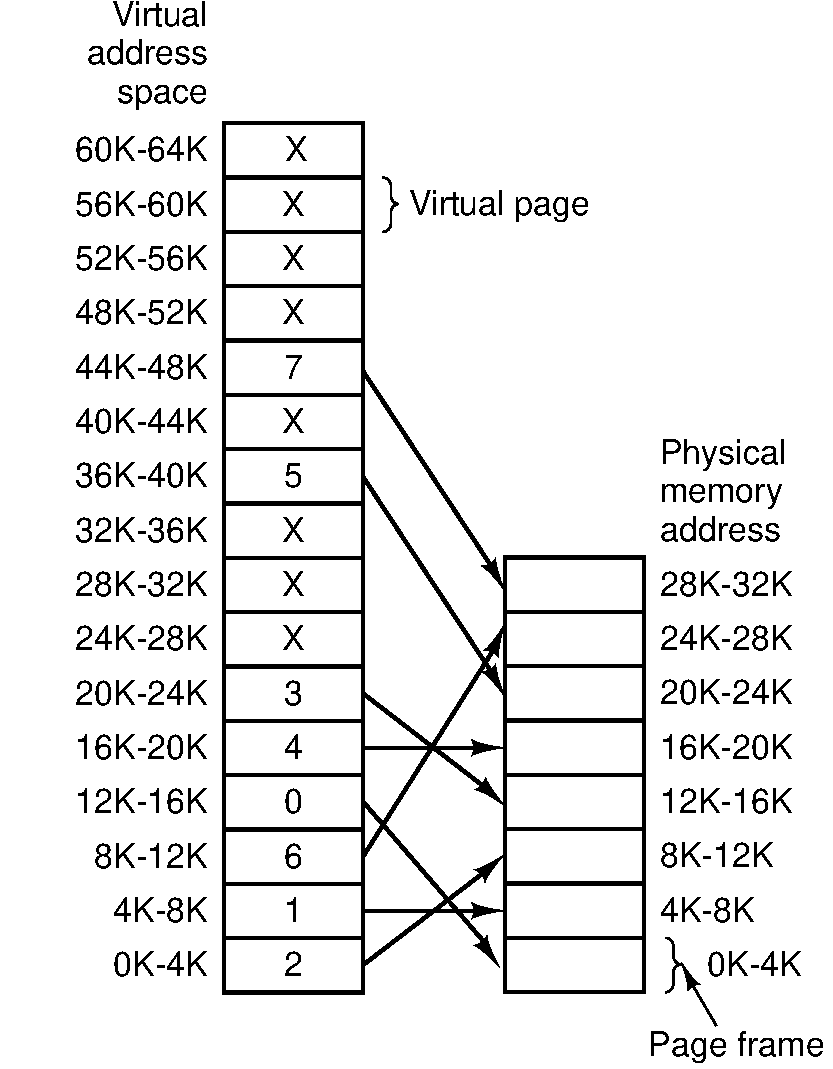
\includegraphics[width=.8\textwidth]{mos-figs-4-10} }
    \end{center}
  \end{varwidth}\hfill
  \begin{varwidth}{.48\textwidth}
    \begin{block}{Address translation}
      $$\genfrac{}{}{0pt}{}{virtual}{address}
      \xrightarrow{\alert{page\,table}}
      \genfrac{}{}{0pt}{}{physical}{address}$$
      
      $$Page\ 0\xrightarrow{map\,to}Frame\ 2$$
      
      $$0_{virtual}\xrightarrow{map\,to}8192_{physical}$$
      
      $$\genfrac{}{}{0pt}{}{20500_{vir}}{(20k+20)_{vir}}
      \xrightarrow{map\,to} \genfrac{}{}{0pt}{}{12308_{phy}}{(12k+20)_{phy}}$$
    \end{block}
  \end{varwidth}
\end{frame}

\begin{frame}{Paging}{Address Translation Scheme}
  \begin{block}{Address generated by CPU is divided into:}
    \begin{description}
    \item[Page number(p):] an index into a page table
    \item[Page offset(d):] to be copied into memory
    \end{description}
  \end{block}
  Given \alert{logical address space} ($2^m$) and \alert{page size} ($2^n$),
  \begin{small}
    $$\text{number of pages}=\frac{2^m}{2^n}=2^{m-n}$$
  \end{small}
  \begin{block}{Example: addressing to $0010000000000100$}
    $$\underbrace{\overbrace{0\,0\,1\,0}^{m-n=4}\,\overbrace{0\,0\,0\,0\,0\,0\,0\,0\,0\,1\,0\,0}^{n=12}}_{m=16}$$
    \begin{small}
      $$\text{page number}=0010=2, \quad \text{page offset}=000000000100$$
    \end{small}
  \end{block}
\end{frame}

\begin{frame}
  \begin{varwidth}{.65\textwidth}
    \begin{center}
      \mode<beamer>{ 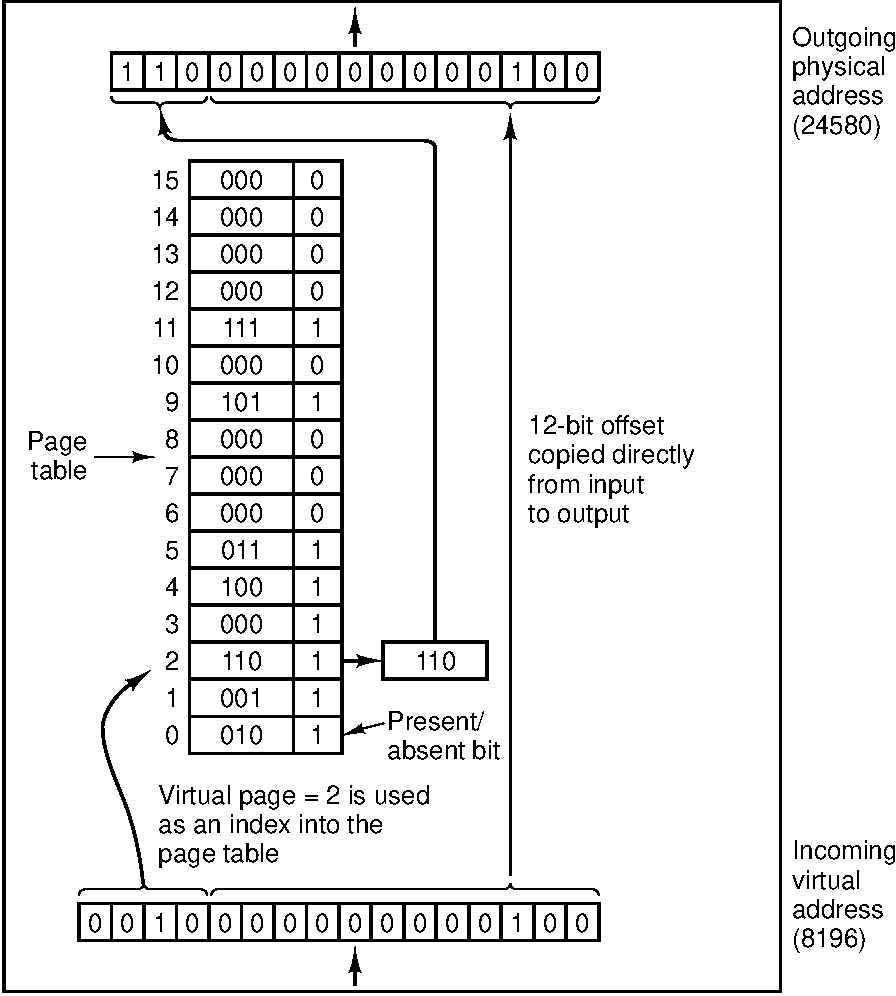
\includegraphics[width=\textwidth]{mos-figs-4-11} }%
      \mode<article>{ 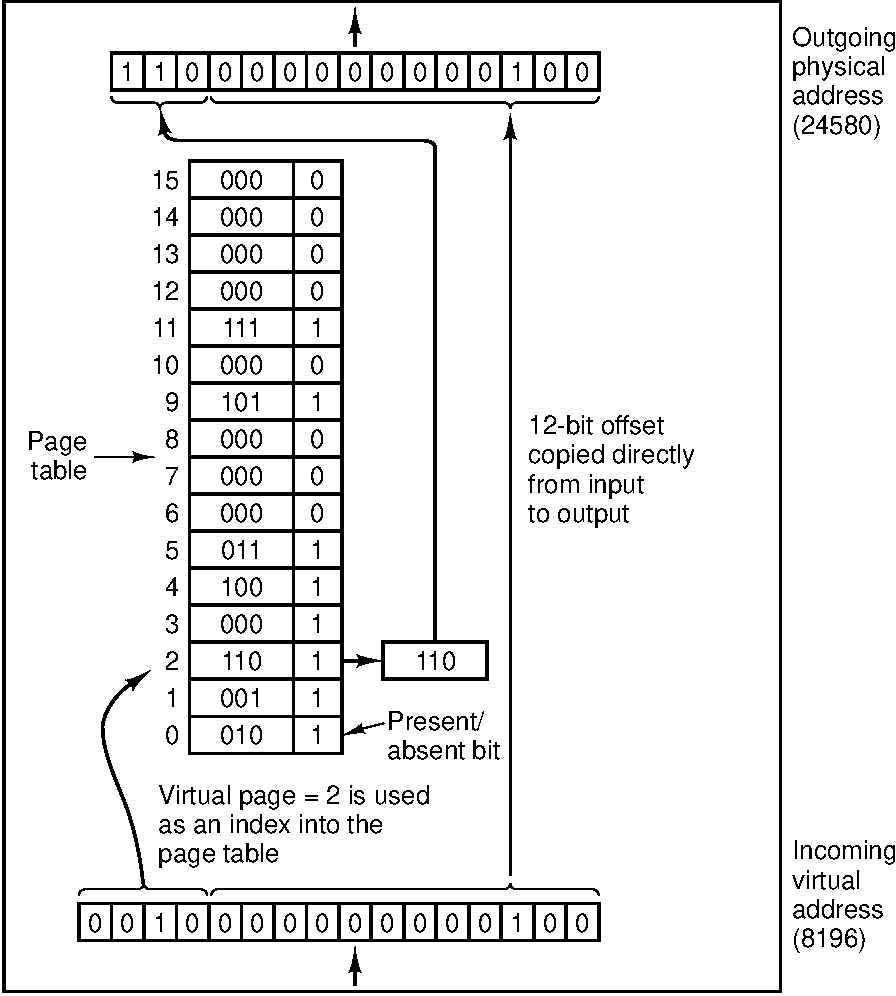
\includegraphics[width=.8\textwidth]{mos-figs-4-11} }
    \end{center}
    \label{fig:paging}
  \end{varwidth}\hfill
  \begin{varwidth}{.35\textwidth}
    \begin{small}
      \begin{tabular}{rl}
        Virtual pages:  &16\\
        Page size:      &4k\\
        Virtual memory: & 64K\\
        Physical frames:&8\\
        Physical memory:&32K
      \end{tabular}
    \end{small}
  \end{varwidth}
\end{frame}

\begin{frame}[fragile]{Page Fault}
  \begin{varwidth}{.48\textwidth}
    \begin{center}
      \mode<beamer>{ 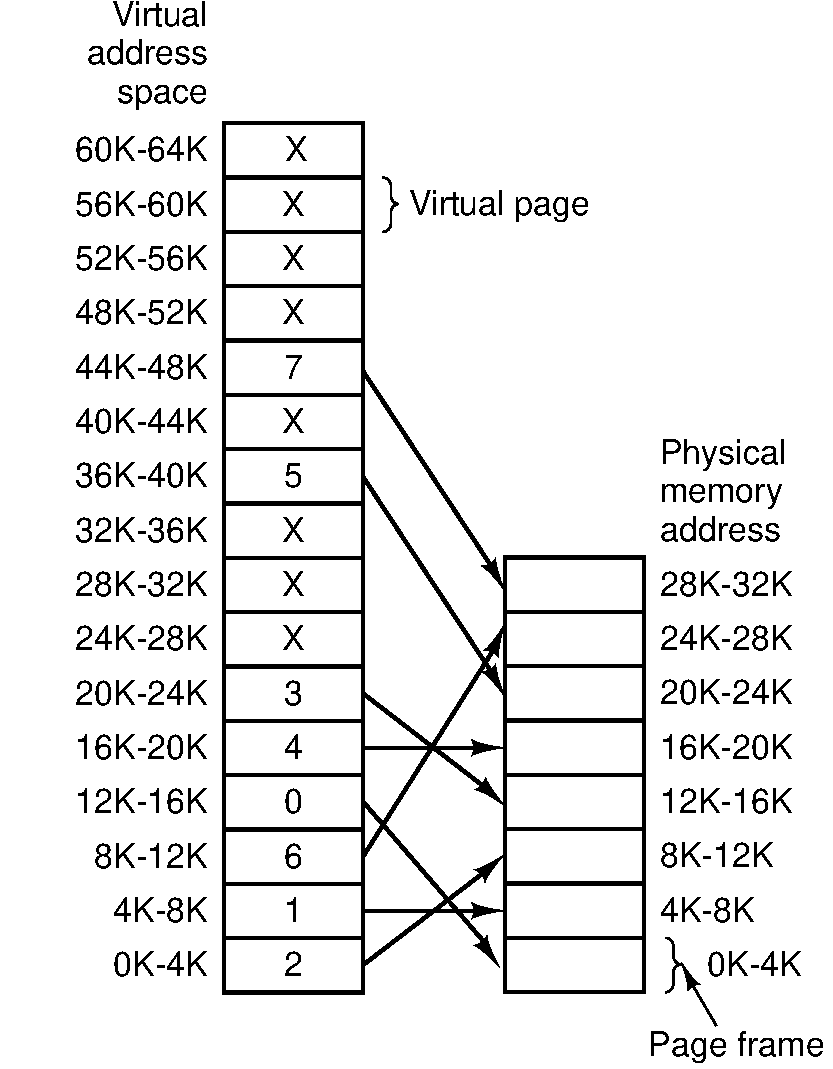
\includegraphics[width=\textwidth]{mos-figs-4-10} }%
      \mode<article>{ 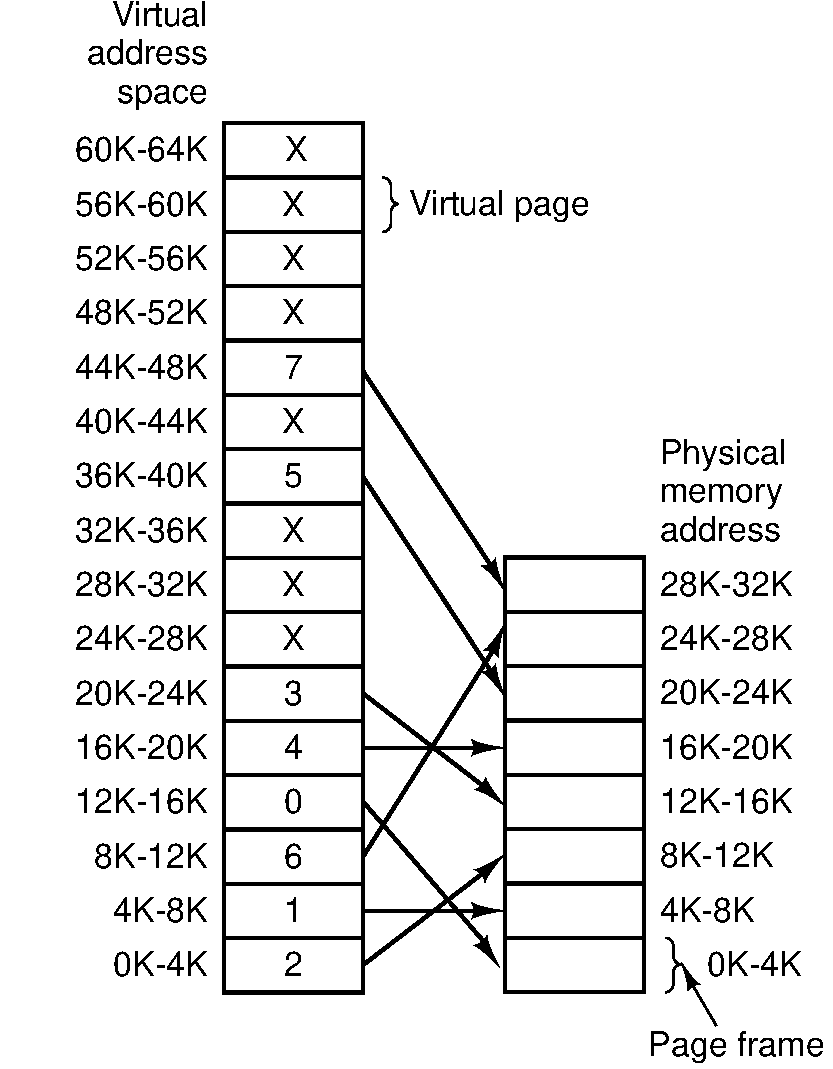
\includegraphics[width=.8\textwidth]{mos-figs-4-10} }
    \end{center}
  \end{varwidth}\hfill
  \begin{varwidth}{.48\textwidth}
    \mintinline{nasm}|MOV REG, 32780|?
    \begin{itemize}
    \item[\Symbol{➠}] Page fault \& swapping
    \end{itemize}
  \end{varwidth}
\end{frame}

\begin{frame}{Page Fault Handling}
  \begin{center}
    \mode<beamer>{ 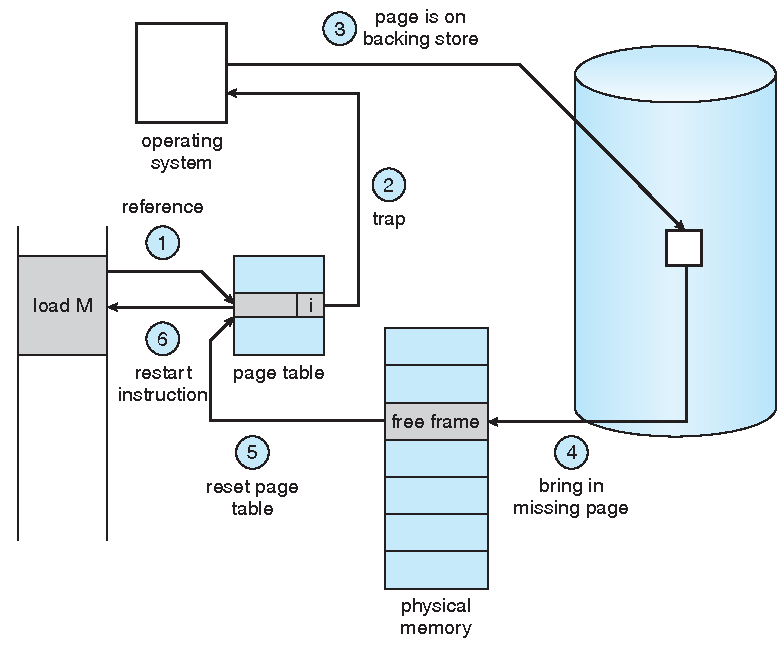
\includegraphics[width=.8\textwidth]{osc-9-14} }%
    \mode<article>{ 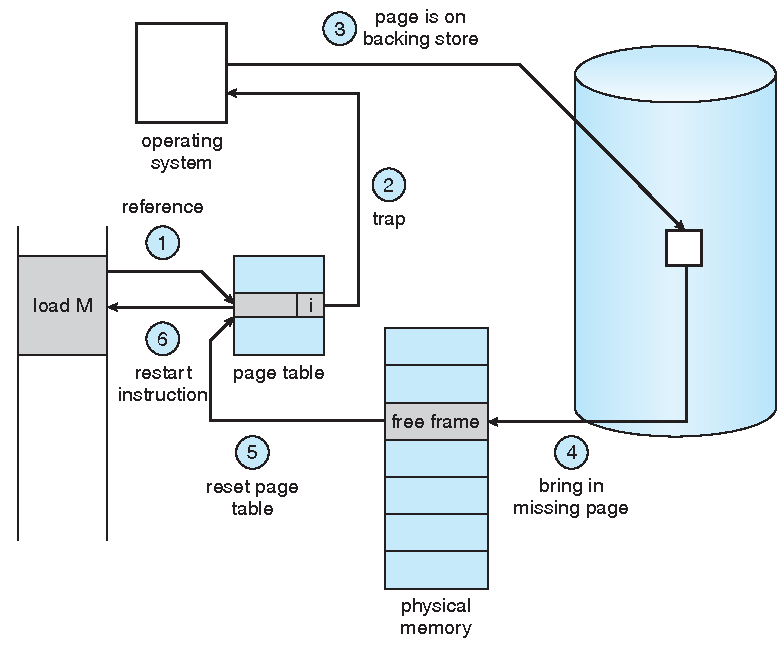
\includegraphics[width=.4\textwidth]{osc-9-14} }
  \end{center}
\end{frame}

\begin{frame}{Shared Pages}
  \begin{center}
    \mode<beamer>{ 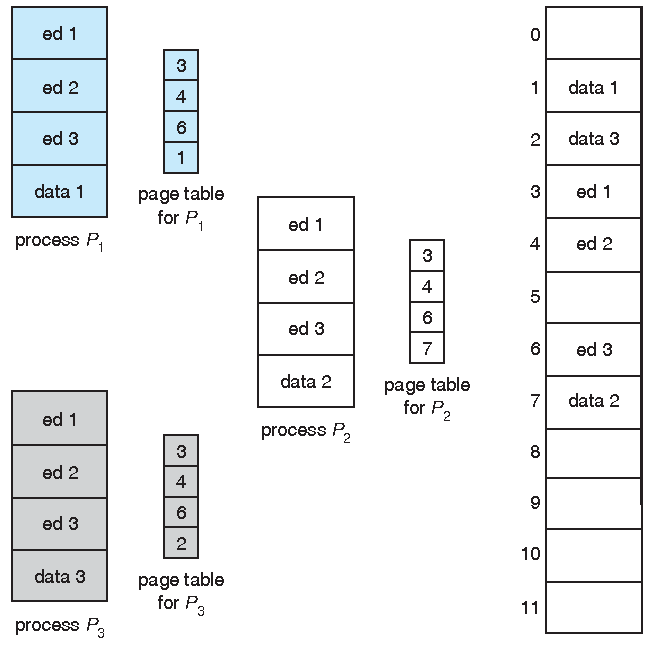
\includegraphics[width=.7\textwidth]{osc-8-33} }%
    \mode<article>{ 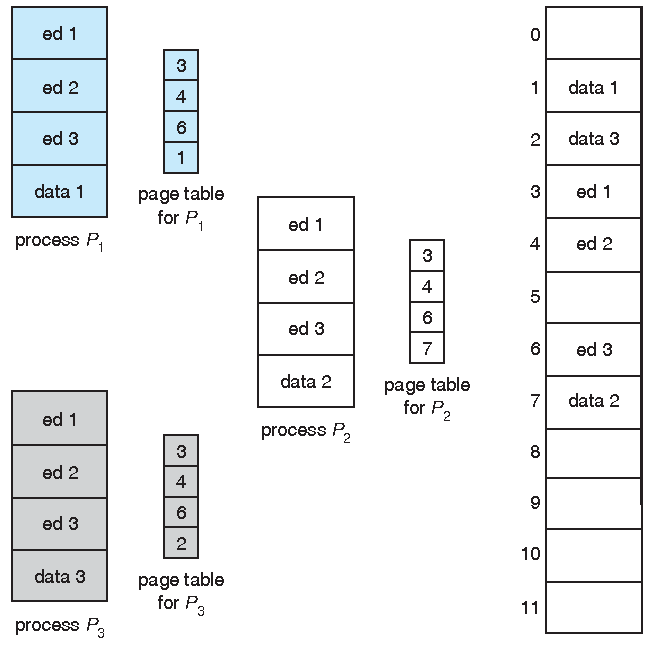
\includegraphics[width=.4\textwidth]{osc-8-33} }
  \end{center}
\end{frame}

\begin{frame}{Page Table Entry}{Intel i386 Page Table Entry}
  \begin{itemize}
  \item Commonly 4 bytes (32 bits) long
  \item Page size is usually 4k ($2^{12}$ bytes). OS dependent
    \begin{itemize}
    \item[\$] \texttt{getconf PAGESIZE}
    \end{itemize}
  \item Could have $2^{32-12}=2^{20}=1M$ pages
    \begin{itemize}
    \item[] Could address $1M\times{}4KB=4GB$ memory
    \end{itemize}
  \end{itemize}
  \begin{center}
    \mode<beamer>{ \includegraphics[width=.9\textwidth]{i386pte} }%
    \mode<article>{ \includegraphics[width=.5\textwidth]{i386pte} }
  \end{center}
\end{frame}

\begin{frame}{Page Table}
  \begin{itemize}
  \item Page table is kept in main memory
  \item Usually one page table for each process
  \item \alert{Page-table base register (PTBR):} A pointer to the page table is stored in
    PCB
  \item \alert{Page-table length register (PRLR):} indicates size of the page table
  \item Slow
    \begin{itemize}
    \item Requires two memory accesses. One for the page table and one for the
      data/instruction.
    \end{itemize}
  \item TLB
  \end{itemize}
\end{frame}

\begin{frame}{Translation Lookaside Buffer (TLB)}
  \begin{description}
  \item[80-20 rule] Only a small fraction of the PTEs are heavily read; the rest are
    barely used at all
  \end{description}
  \begin{center}
    \mode<beamer>{ 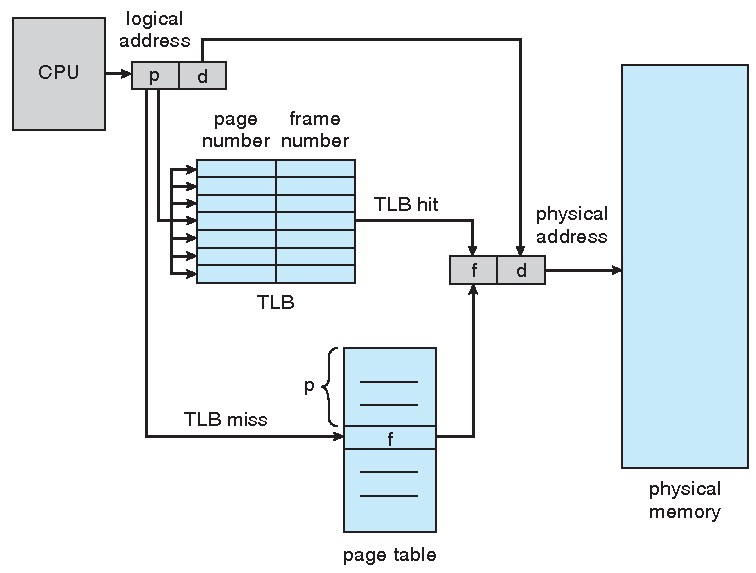
\includegraphics[width=.7\textwidth]{osc-8-28} }%
    \mode<article>{ 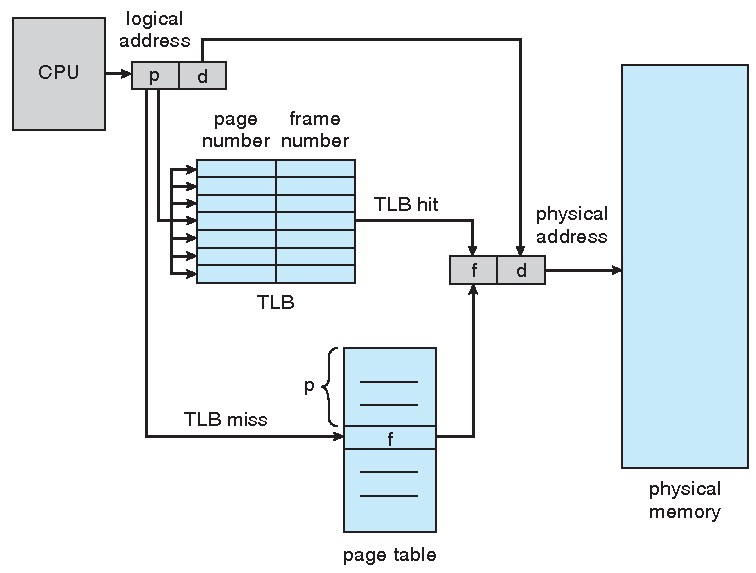
\includegraphics[width=.5\textwidth]{osc-8-28} }
  \end{center}
\end{frame}

\begin{frame}{Multilevel Page Tables}
  \begin{itemize}
  \item a $1M$-entry page table eats $4M$ memory
  \item while 100 processes running, $400M$ memory is gone for page tables
  \item avoid keeping all the page tables in memory all the time
  \end{itemize}
  \begin{block}{A two-level scheme}
    \begin{center}
      \mode<beamer>{ 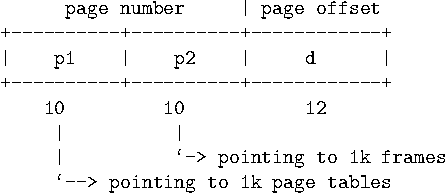
\includegraphics[width=.6\textwidth]{2-level-paging} }%
      \mode<article>{ 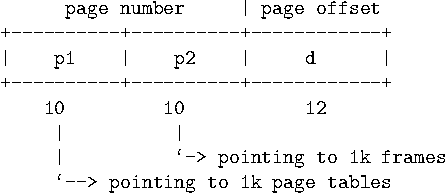
\includegraphics[width=.3\textwidth]{2-level-paging} }
    \end{center}
  \end{block}
\end{frame}

\begin{description}
\item[p1:] is an index into the outer page table
\item[p2:] is the displacement within the page of the outer page table
\end{description}

\begin{itemize}
\item Split one huge page table into 1k small page tables
  \begin{itemize}
  \item i.e. the huge page table has 1k entries.
  \item Each entry keeps a page frame number of a small page table.
  \end{itemize}
\item Each small page table has 1k entries
  \begin{itemize}
  \item Each entry keeps a page frame number of a physical frame.
  \end{itemize}
\end{itemize}

\begin{frame}{Two-Level Page Tables}{Example}
  \begin{center}
    \mode<beamer>{ 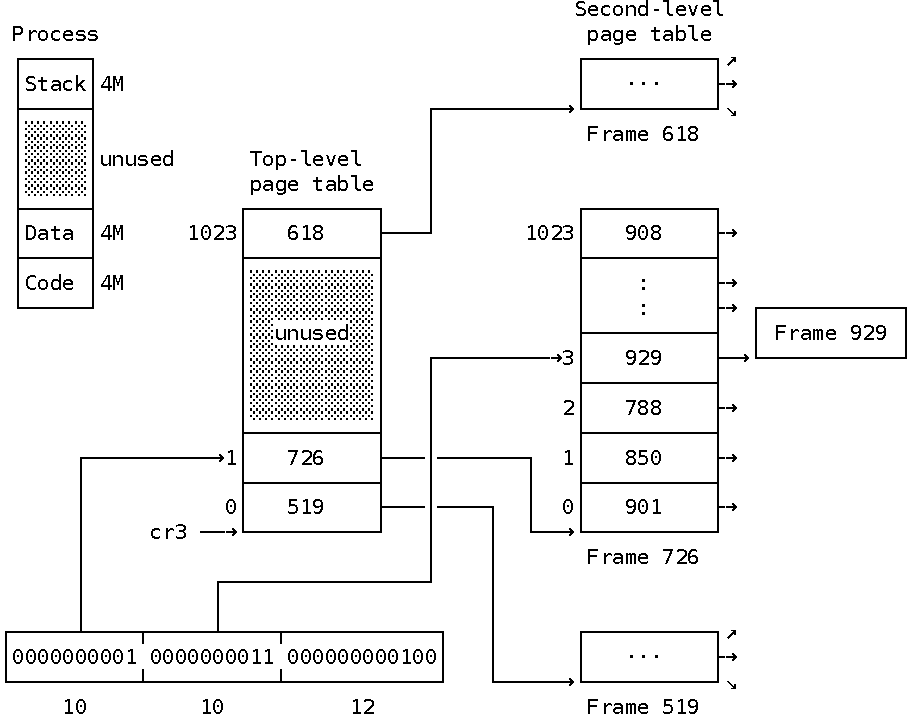
\includegraphics[width=.8\textwidth]{2-level-paging-2} }%
    \mode<article>{ 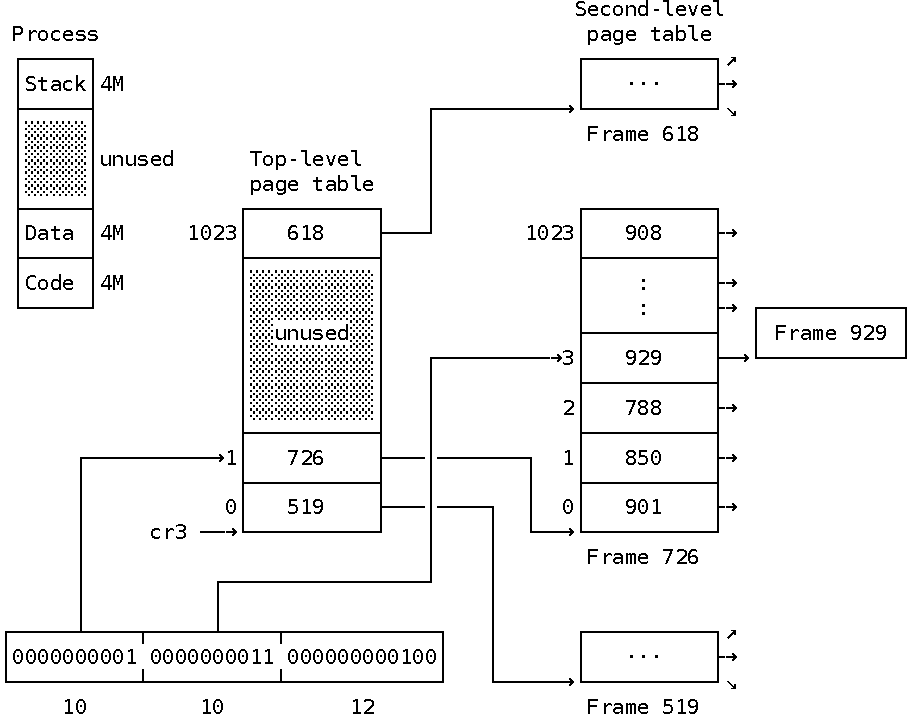
\includegraphics[width=.6\textwidth]{2-level-paging-2} }
  \end{center}
\end{frame}

\begin{frame}{Pentium Paging}{Linear Address $\Rightarrow$ Physical Address}
  \begin{minipage}{.4\textwidth}
    \mbox{Two page size in Pentium:}
    \begin{small}
      \begin{itemize}
      \item[4K:] \mbox{2-level paging}% (Fig.~\ref{fig:2levelpaging})}
      \item[4M:] \mbox{1-level paging}% (Fig.~\ref{fig:paging})}
      \end{itemize}
    \end{small}
    \begin{center}
      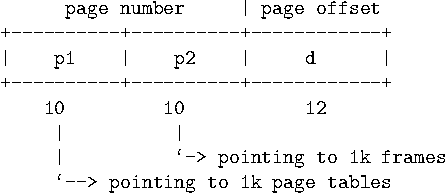
\includegraphics[width=1.15\textwidth]{2-level-paging}
    \end{center}
  \end{minipage}\quad
  \begin{minipage}{.5\textwidth}
    \begin{center}
      \mode<beamer>{ 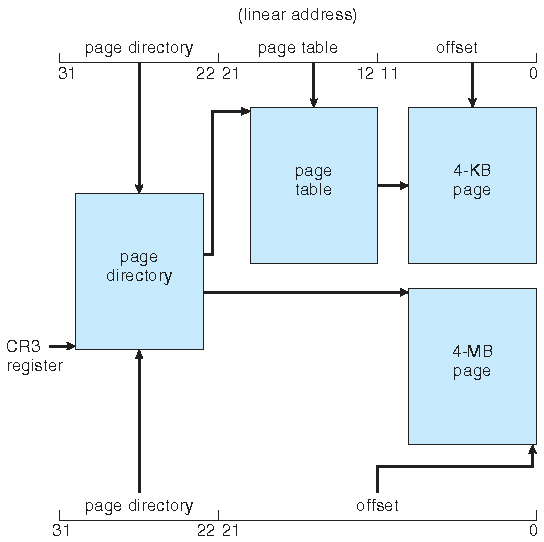
\includegraphics[width=1.1\textwidth]{osc-8-54} }%
      \mode<article>{ 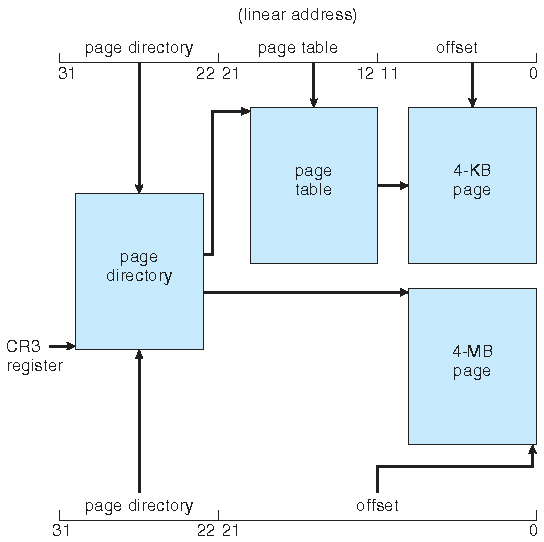
\includegraphics[width=.8\textwidth]{osc-8-54} }
    \end{center}
  \end{minipage}
\end{frame}

\begin{frame}{Problem With 64-bit Systems}
  \begin{description}
  \item[Given:]\hfill\\[-2ex]
    \begin{itemize}
    \item $\text{virtual address space} = 64\,bits$
    \item $\text{page size}=4\,KB=2^{12}\,B$
    \end{itemize}
  \item[?] How much space would a simple single-level page table take?
    \begin{itemize}
    \item[if] Each page table entry takes $4\,Bytes$
    \item[then] The whole page table ($2^{64-12}$ entries) will take
      \[2^{64-12}\times{}4\,B=2^{54}\,B=16\,PB \quad {\scriptstyle(peta \Rightarrow tera \Rightarrow giga)!}\]
    \end{itemize}
    And this is for ONE process!
  \item[Multi-level?]\hfill
    \begin{itemize}
    \item[if] $10\,bits$ for each level
    \item[then] $\frac{64-12}{10}=5$ levels are required
    \end{itemize}
    5 memory accress for each address translation!
  \end{description}
\end{frame}

\begin{itemize}
\item The CR3 register {\pright} the top level page table for the current process.
\end{itemize}

\begin{frame}{Paging In Linux}{4-level paging for both 32-bit and 64-bit}
  \begin{center}
    \mode<beamer>{ 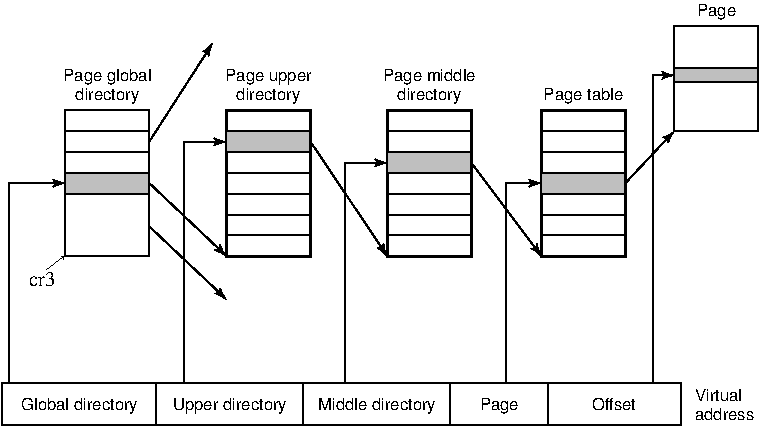
\includegraphics[width=\textwidth]{4-level-paging} }%
    \mode<article>{ 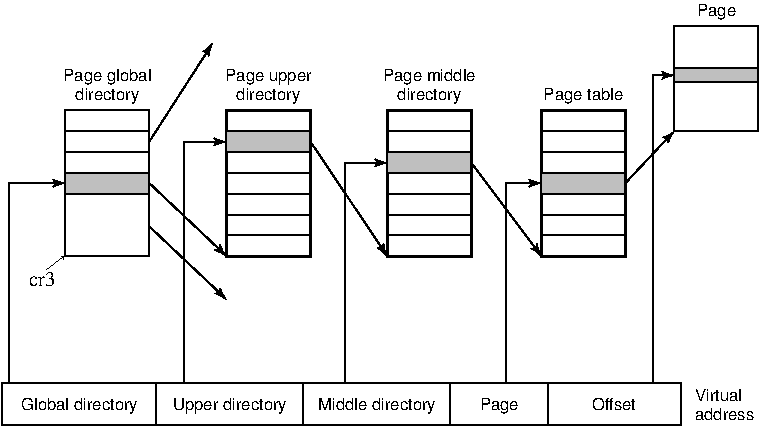
\includegraphics[width=.5\textwidth]{4-level-paging} }
  \end{center}
\end{frame}

\begin{frame}%{Paging In Linux}
  \begin{block}{4-level paging for both 32-bit and 64-bit}
    \begin{itemize}
    \item \alert{64-bit: four-level paging}
      \begin{enumerate}
      \item Page Global Directory
      \item Page Upper Directory
      \item Page Middle Directory
      \item Page Table
      \end{enumerate}
    \item \alert{32-bit: two-level paging}
      \begin{enumerate}
      \item Page Global Directory
      \item Page Upper Directory --- 0 bits; 1 entry
      \item Page Middle Directory --- 0 bits; 1 entry
      \item Page Table
      \end{enumerate}
    \end{itemize}
    \alert{The same code can work on 32-bit and 64-bit architectures}
  \end{block}
    \begin{center}
    \begin{scriptsize}
      \begin{tabular}{llm{3em}m{3em}r}
        \hline
        Arch&Page size&Address bits&Paging levels&Address splitting\\\hline
        x86 &4KB(12bits) &32 &2 &$10+0+0+10+12$\\
        x86-PAE&4KB(12bits)&32&3&$2+0+9+\hspace{.6em}9+12$\\
        x86-64&4KB(12bits)&48&4&$9+9+9+\hspace{.6em}9+12$\\\hline
      \end{tabular}
    \end{scriptsize}
  \end{center}
\end{frame}


\section{Process}
\label{sec:process}

\begin{frame}
  \begin{block}{From kernel's point of view}
    A process consists of
    \begin{description}
    \item[User-space memory] program code, variable...
    \item[Kernel data structures] keep the state of the process
    \end{description}
  \end{block}
\end{frame}

\begin{frame}{Process Control Block (PCB)}
  \begin{varwidth}{.7\textwidth}
    \begin{block}{Implementation}
        A process is \alert{the collection of data structures} that fully describes how far
        the execution of the program has progressed.
        \begin{itemize}
        \item Each process is represented by a \alert{PCB}
        \item \texttt{task\_struct} in \linux{}
        \end{itemize}
      \end{block}
    \end{varwidth}\quad
    \begin{varwidth}{.2\textwidth}
      \begin{center}
        \mode<beamer>{ \includegraphics[width=1.5\textwidth]{pcb} }%
        \mode<article>{ \includegraphics[width=\textwidth]{pcb} }
      \end{center}      
    \end{varwidth}
\end{frame}

\begin{frame}{Process Creation}
  \begin{center}
    \mode<beamer>{ 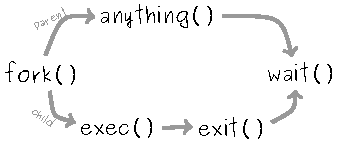
\includegraphics[width=\textwidth]{process-creation} }%
    \mode<article>{ 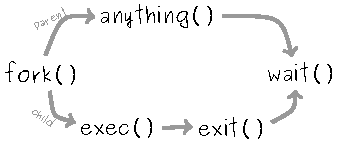
\includegraphics[width=.4\textwidth]{process-creation} }
  \end{center}
  \begin{itemize}
  \item When a process is created, it is almost identical to its parent
    \begin{itemize}
    \item It receives a (logical) copy of the parent's address space, and
    \item executes the same code as the parent
    \end{itemize}
  \item The parent and child have separate copies of the data (stack and heap)
  \end{itemize}
\end{frame}

\begin{frame}{Process State Transition}
  \begin{center}
    \mode<beamer>{ 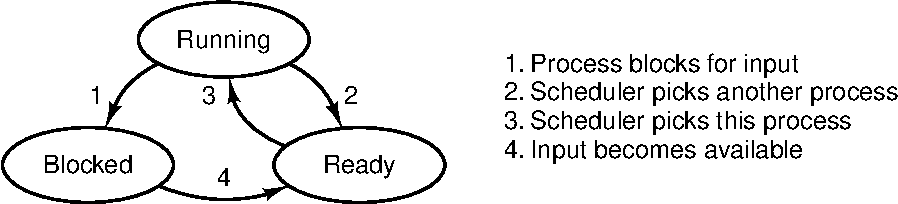
\includegraphics[width=\textwidth]{mos-figs-2-2} }%
    \mode<article>{ 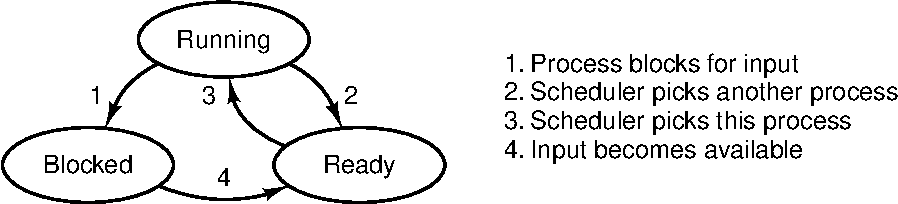
\includegraphics[width=.7\textwidth]{mos-figs-2-2} }
  \end{center}
\end{frame}

\begin{frame}{CPU Switch From Process To Process}
  \begin{center}
    \mode<beamer>{ 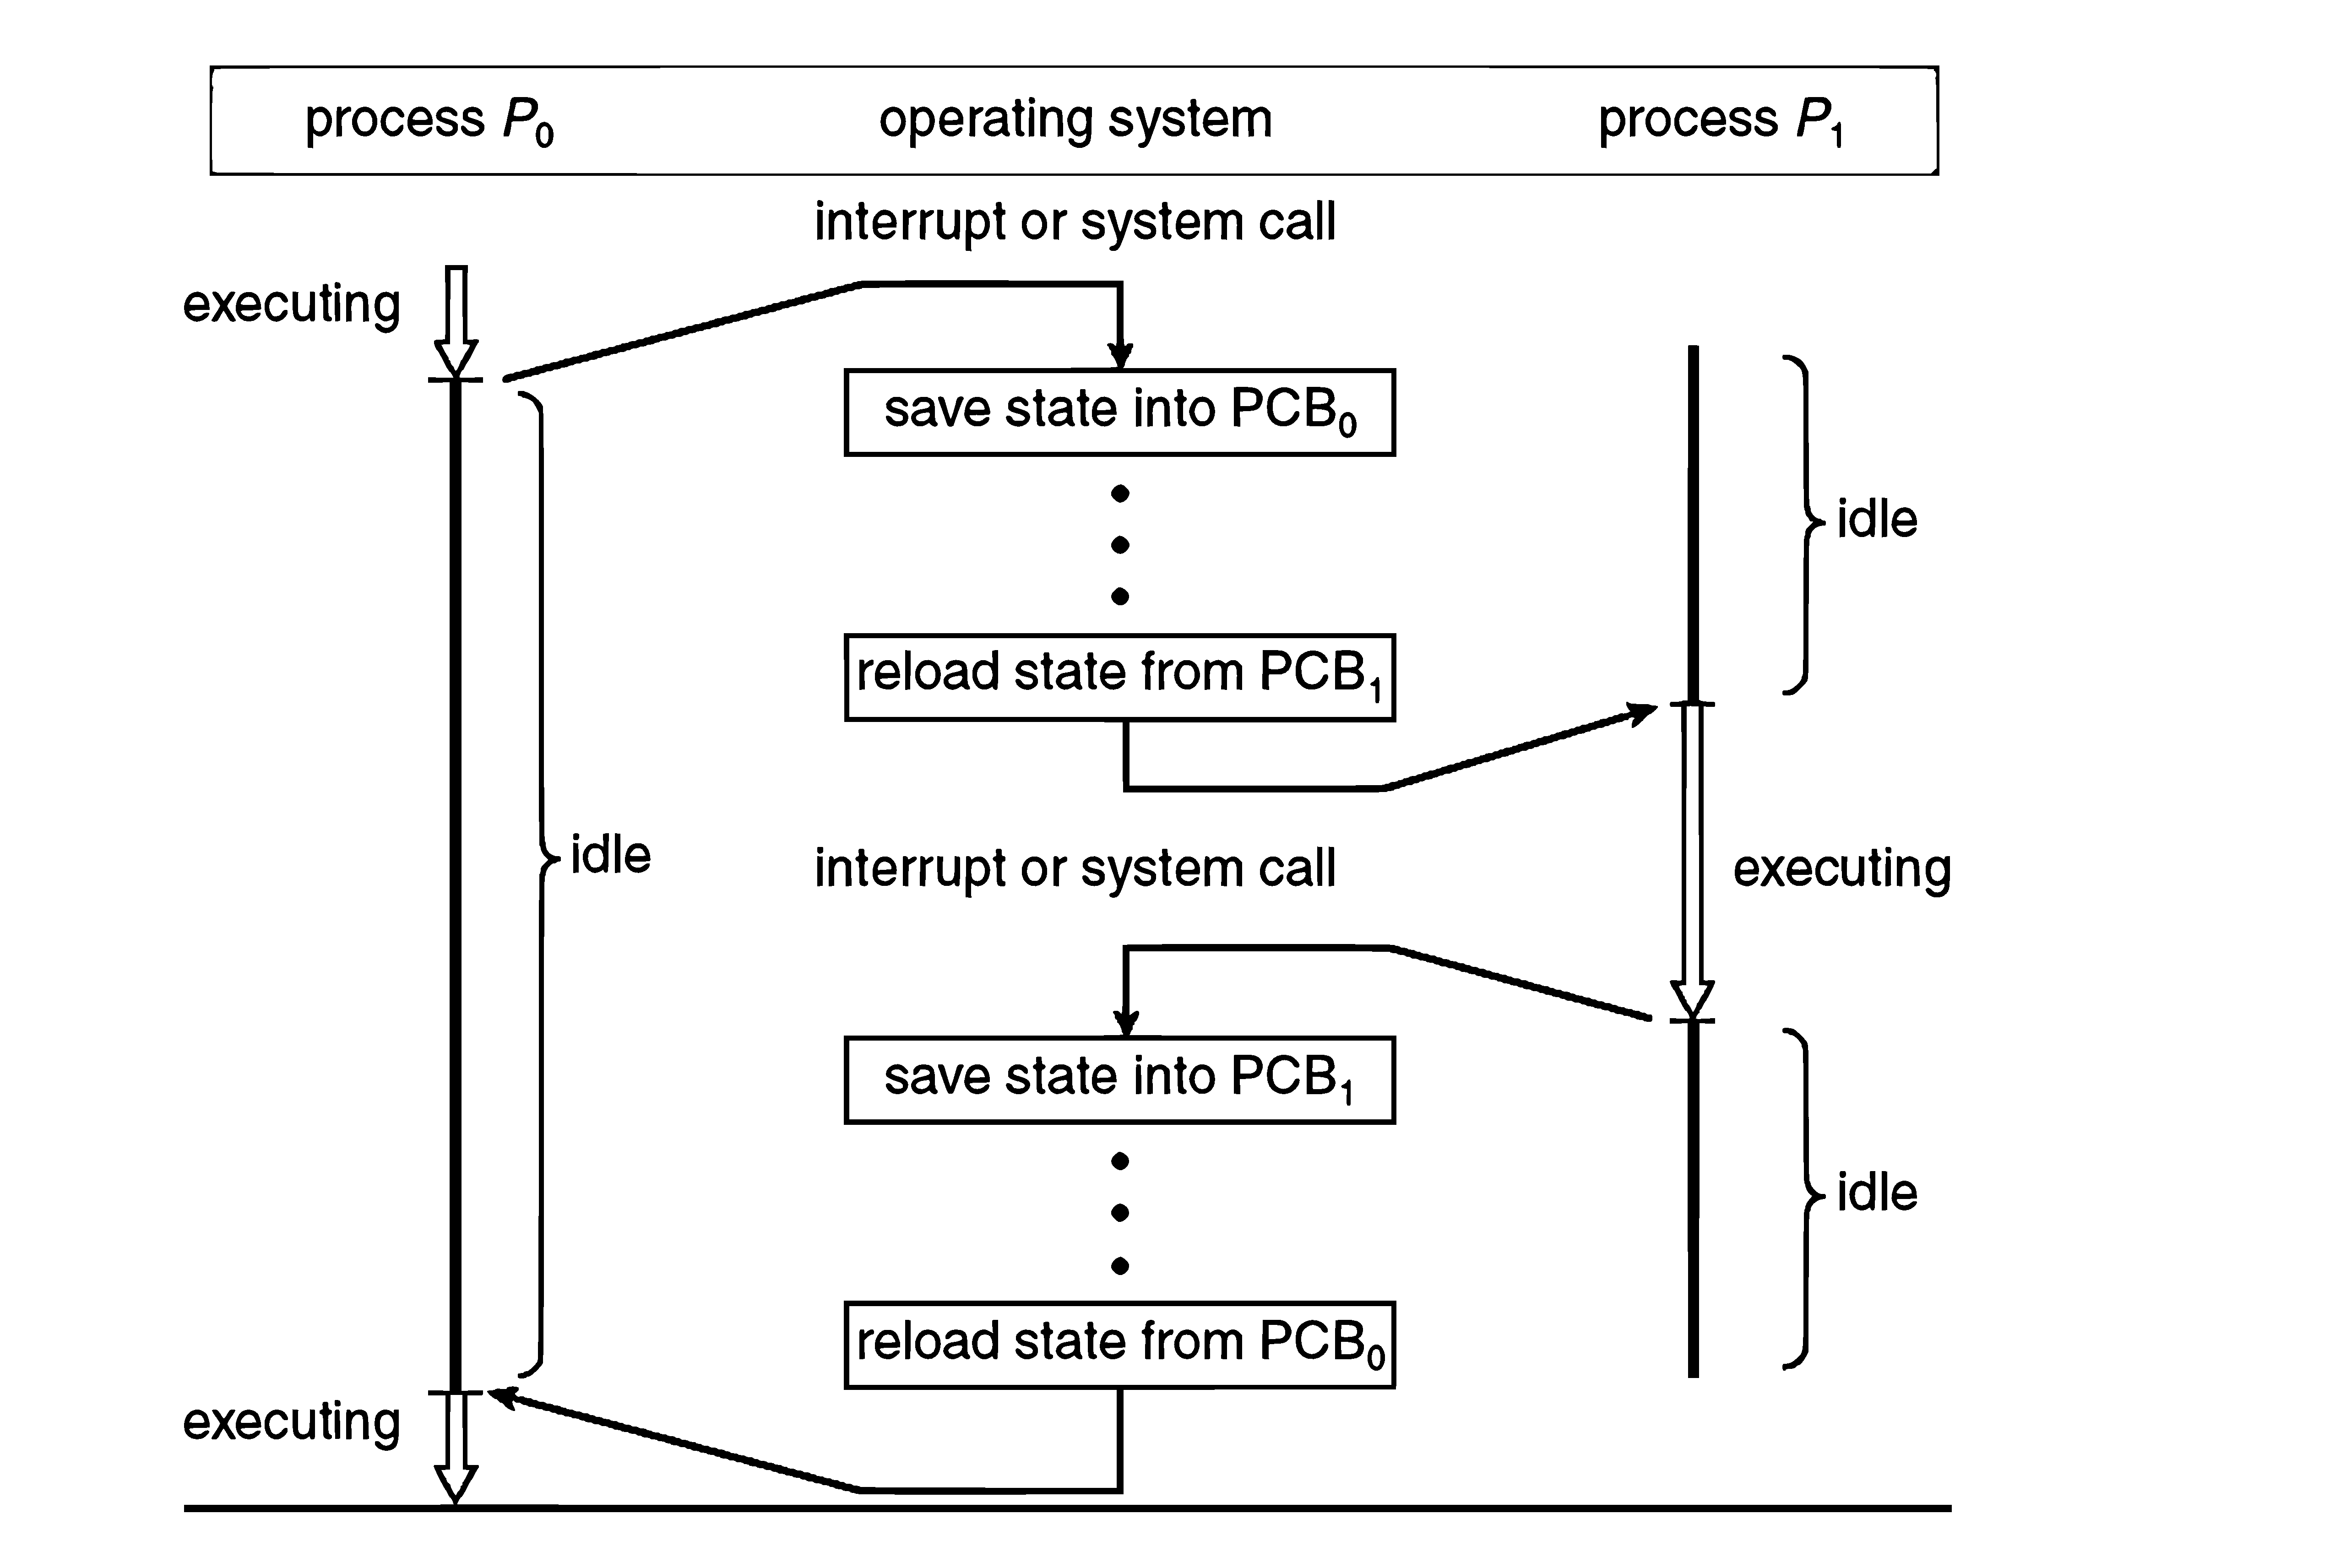
\includegraphics[width=\textwidth]{cpu-switch} }%
    \mode<article>{ 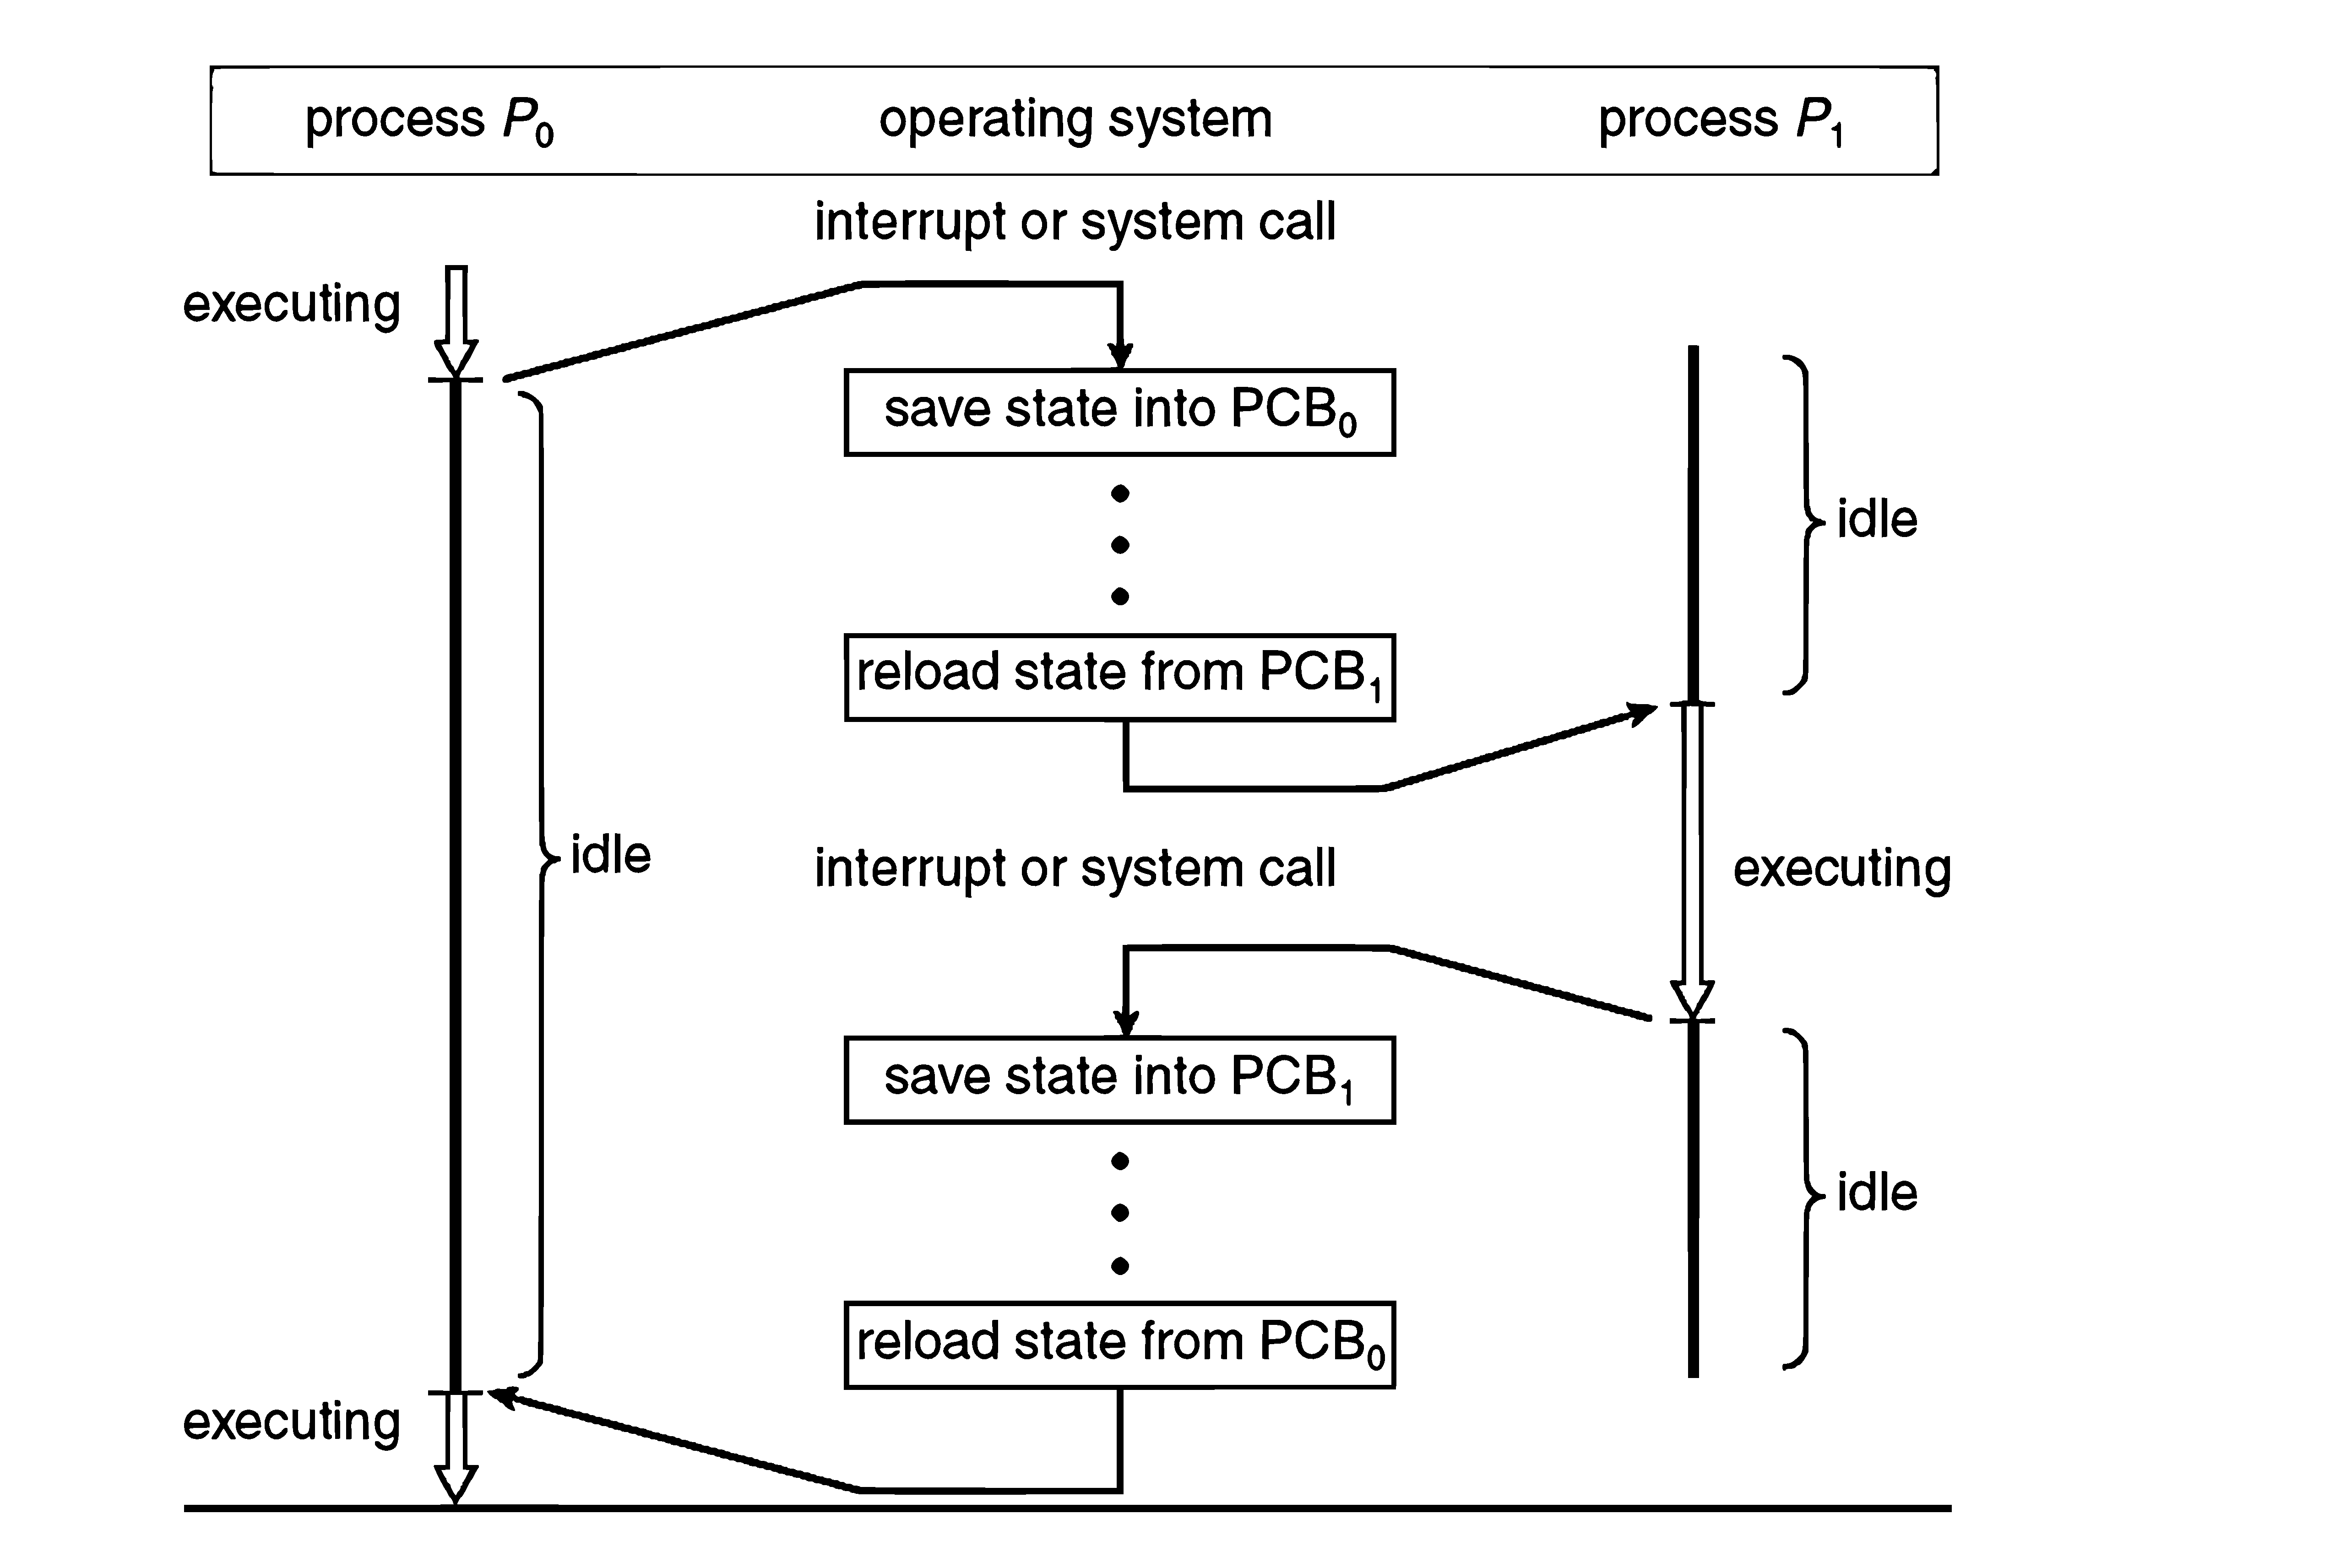
\includegraphics[width=.7\textwidth]{cpu-switch} }
  \end{center}
\end{frame}

\begin{frame}{Forking in C}
  \begin{center}
    \mode<beamer>{ 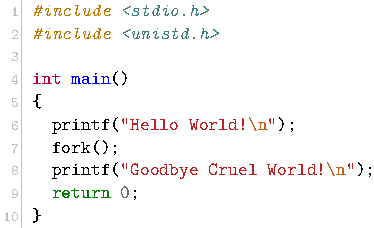
\includegraphics[width=.7\textwidth]{fork} }%
    \mode<article>{ \includegraphics[width=.4\textwidth]{fork-bw} }
  \end{center}
\end{frame}

\begin{frame}{\texttt{exec()}}
  \begin{center}
    \mode<beamer>{ 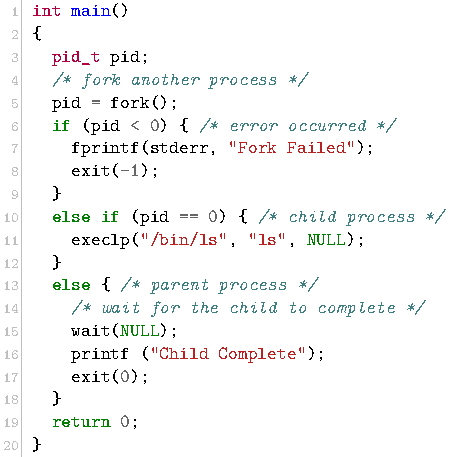
\includegraphics[width=.7\textwidth]{fork-exec-osc} }%
    \mode<article>{ 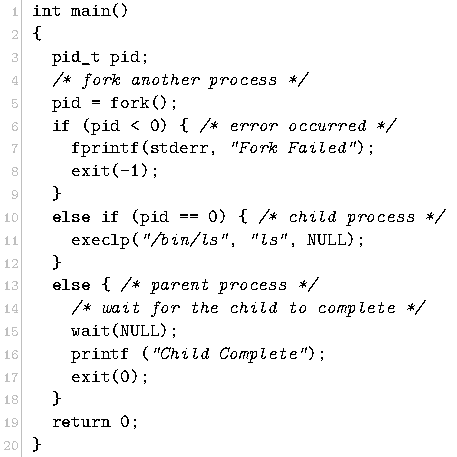
\includegraphics[width=.4\textwidth]{fork-exec-osc-bw} }
  \end{center}
\end{frame}

\paragraph{More about \texttt{argv[0]}}

\texttt{int execve(const char *pathname, char *const argv[], char *const envp[]);}
\begin{itemize}
\item \texttt{pathname} should be the binary image of a program. Or it can be a script
  (\cmd{man 2 execve});
\item \texttt{argv[0]} is the new process name, usually the same as the basename of
  \texttt{pathname}, though it can be any other string. It can even be NULL (see
  Figure~\ref{fig:argv0} for example).

  The fact that \texttt{argv[0]} contains the name used to invoke the program can be
  employed to perform a useful trick. We can create multiple links to (i.e., names for)
  the same program, and then have the program look at \texttt{argv[0]} and take different
  actions depending on the name used to invoke it. An example of this technique is
  provided by the \emph{gzip(1)}, \emph{gunzip(1)}, and \emph{zcat(1)} commands, all of
  which are links to the same executable
  file. \citetitle[Sec.~6.6]{Kerrisk:2010:LPI:1869911}
\item \url{https://stackoverflow.com/questions/2794150/when-can-argv0-have-null}
\item \url{https://stackoverflow.com/questions/36673765/why-can-the-execve-system-call-run-bin-sh-without-any-argv-arguments-but-not}
\end{itemize}

\begin{figure}
  \centering
  \begin{minipage}{.4\linewidth}
    \begin{center}
      \cfile{../src/caller.c}
      % \includegraphics[width=\textwidth]{caller-c-bw}
      \caption{\texttt{caller.c}}
    \end{center}
  \end{minipage}\qquad
  \begin{minipage}{.4\linewidth}
    \begin{center}
      \cfile{../src/callee.c}
      % 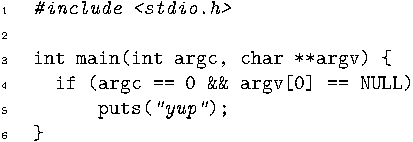
\includegraphics[width=\textwidth]{callee-c-bw}
      \caption{\texttt{callee.c}}
    \end{center}
  \end{minipage}\\[1em]
  \ttfamily
  \begin{itemize}
  \item[\$] gcc -Wall caller.c -o caller.out
  \item[\$] gcc -Wall callee.c -o callee.out
  \item[\$] ./caller.out ./callee.out
  \end{itemize}
  \caption{\texttt{argv[0]} can be NULL}
  \label{fig:argv0}
\end{figure}

% \subsection{Sessions and Process Groups}

% \begin{frame}\ttfamily
%   \begin{itemize}
%   \item[\$] find / 2> /dev/null | wc -l \&
%   \item[\$] sort < longlist | uniq -c
%   \end{itemize}
% \begin{center}
%   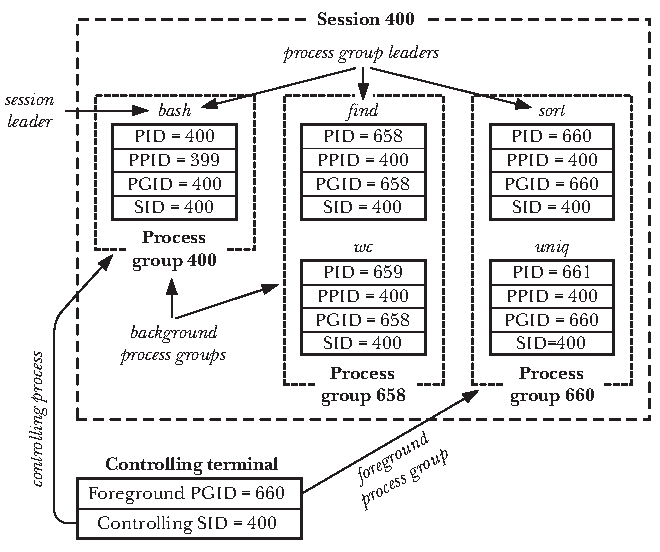
\includegraphics[width=.6\textwidth]{session}
% \end{center}

% \end{frame}

\section{Thread}
\label{sec:thread}

\begin{frame}{Process vs. Thread}
    \begin{tabular}{r@{\quad{}=\quad}l}
      a single-threaded process&resource + execution\\
      a  multi-threaded process&resource + executions\\
    \end{tabular}
    \begin{center}
      \mode<beamer>{ \includegraphics[width=.7\textwidth]{mos-figs-2-6} }%
      \mode<article>{ \includegraphics[width=.6\textwidth]{mos-figs-2-6} }
    \end{center}
  \begin{description}
  \item[A process] = a unit of resource ownership, used to group resources together;
  \item[A thread] = a unit of scheduling, scheduled for execution on the CPU.
  \end{description}  
\end{frame}

\begin{frame}{Threads}
  \begin{center}
    \mode<beamer>{ \includegraphics[width=.8\textwidth]{thread-components} }%
    \mode<article>{ \includegraphics[width=.4\textwidth]{thread-components} }
  \end{center}
\end{frame}

\begin{frame}{POSIX Threads}
  \begin{description}
  \item[IEEE 1003.1c] The standard for writing portable threaded programs. The threads package it
    defines is called \alert{Pthreads}, including over 60 function calls, supported by most UNIX
    systems.
  \end{description}
  \begin{block}{Some of the Pthreads function calls}
    \begin{center}
      \begin{small}
        \begin{tabular}{>{\ttfamily}ll}
          \hline
          \thead{Thread call}&\thead{Description}\\\hline
          pthread\_create&Create a new thread\\
          pthread\_exit&Terminate the calling thread\\
          pthread\_join&Wait for a specific thread to exit\\
          pthread\_yield&Release the CPU to let another thread run\\
          pthread\_attr\_init&Create and initialize a thread's attribute structure\\
          pthread\_attr\_destroy&Remove a thread's attribute structure\\\hline
        \end{tabular}
      \end{small}
    \end{center}
  \end{block}
\end{frame}

\begin{frame}{Pthreads}{Example 1}
  \begin{center}
    \mode<beamer>{ \includegraphics[width=.7\textwidth]{thread1} }%
    \mode<article>{\cfile{../src/thread1.c}}
  \end{center}
\end{frame}

\begin{frame}{Pthreads}
  \begin{description}
  \item[\texttt{pthread\_t}] defined in \texttt{pthread.h}, is often called a "thread id"
    (\texttt{tid});
  \item[\texttt{pthread\_create()}] returns zero on success and a non-zero value on failure;
  \item[\texttt{pthread\_join()}] returns zero on success and a non-zero value on failure;
  \end{description}
  \begin{block}{How to use pthread?}
    \begin{itemize}
    \item \texttt{\#include<pthread.h>}
    \item[\$] \texttt{gcc thread1.c -o thread1 -pthread}
    \item[\$] \texttt{./thread1}
    \end{itemize}
  \end{block}
\end{frame}

\begin{frame}{Pthreads}{Example 2}
  \begin{center}
    \mode<beamer>{ \includegraphics[width=.9\textwidth]{thread2} }%
    \mode<article>{\cfile{../src/thread2.c}}
  \end{center}
\end{frame}

\begin{frame}{Linux Threads}
  \begin{block}{To the Linux kernel, there is no concept of a thread}
    \begin{itemize}
    \item Linux implements all threads as standard processes
    \item To Linux, a thread is merely a process that shares certain resources with other
      processes
    \item Some OS (MS Windows, Sun Solaris) have cheap threads and expensive processes.
    \item Linux processes are already quite lightweight
      \begin{itemize}
      \item[] On a 75MHz Pentium
        \begin{tabular}{r}
          thread: $1.7\mu{}s$\\
          fork: $1.8\mu{}s$
        \end{tabular}
      \end{itemize}
    \end{itemize}
  \end{block}
\end{frame}

\begin{frame}{Linux Threads}
  \begin{description}
  \item[\texttt{clone()}] creates a separate process that shares the address space of the
    calling process. The cloned task behaves \emph{much like} a separate thread.
  \end{description}
  \begin{center}
    \mode<beamer>{ \includegraphics[width=.55\textwidth]{syscall} }%
    \mode<article>{ \includegraphics[width=.4\textwidth]{syscall} }
  \end{center}
\end{frame}

\begin{frame}{\texttt{clone()}}
  \begin{center}
    \mode<beamer>{ \includegraphics[width=\textwidth]{clone-prototype} }%
    \mode<article>{ \includegraphics[width=.6\textwidth]{clone-prototype-bw} }
  \end{center}
  \begin{small}
    \begin{description}
    \item[arg 1] the function to be executed, i.e. \texttt{fn(arg)}, which returns an \texttt{int};
    \item[arg 2] a pointer {\pright} a (usually malloced) memory space to be used as
      the stack for the new thread;
    \item[arg 3] a set of flags used to indicate how much the calling process is to be
      shared. In fact,
      \begin{itemize}
      \item[]  \texttt{clone(0) == fork()}
      \end{itemize}
    \item[arg 4] the arguments passed to the function.
    \end{description}
    It returns the PID of the child process or -1 on failure.
  \end{small}
  \begin{itemize}
    \item[\$] \texttt{man clone}
  \end{itemize}
\end{frame}

\begin{frame}{The \texttt{clone()} System Call}
  \begin{block}{Some flags:}
    \begin{center}
      \begin{tabular}{>{\ttfamily}ll}
        \hline
        \thead{flag}&\thead{Shared}\\\hline
        CLONE\_FS&File-system info\\
        CLONE\_VM&Same memory space\\
        CLONE\_SIGHAND&Signal handlers\\
        CLONE\_FILES&The set of open files\\\hline
      \end{tabular}
    \end{center}
  \end{block}
  \begin{block}{In practice, one should try to avoid calling \texttt{clone()} directly}
    \begin{itemize}
    \item[] Instead, use a threading library (such as pthreads) which use \texttt{clone()}
      when starting a thread (such as during a call to \texttt{pthread\_create()})
    \end{itemize}
  \end{block}
\end{frame}

\begin{frame}{\texttt{clone()} Example}
  \begin{center}
    \mode<beamer>{
      \includegraphics[width=\textwidth]{clone2}
      \pause
      \begin{tikzpicture}[remember picture, overlay]
        \node [yshift=-7em,xshift=5em,rotate=-20,scale=6,text opacity=0.7,color=red] at
        (current page.center) {\Symbol{✘}};
      \end{tikzpicture}
    } \mode<article>{ \includegraphics[width=.45\textwidth]{clone2-bw-crop} }
  \end{center}
\end{frame}

\begin{frame}[fragile]{Stack Grows Downwards}
\begin{ccode}
child_stack = (void**)malloc(8192) + 8192/sizeof(*child_stack);
\end{ccode}
  \mode<beamer>{
    \begin{tikzpicture}[remember picture, overlay]
      \node [yshift=-0.1em,xshift=9em,rotate=0,scale=12,text opacity=0.7,color=red] at
      (current page.center) {\Symbol{✔}};
    \end{tikzpicture}}
\end{frame}

\section{Signals}
\label{sec:signals}

\begin{itemize}
\item Singals are software interrupts. Every signal has a name (SIGXXXX). Signals are
  classic examples of asynchronous events. They occur at what appear to be random times to
  the process. The process can't simply test a variable (such as \texttt{errno}) to see
  whether a signal has occurred; instead, the process has to tell the kernel ``if and when
  this signal occurs, do the following.'' \citetitle[chap. 10]{stevens2013advanced}
\item Signals are software interrupts sent to a program to indicate that an important
  event has occurred. The events can vary from user requests to illegal memory access
  errors. Some signals, such as the interrupt signal, indicate that a user has asked the
  program to do something that is not in the usual flow of
  control. (\url{https://www.tutorialspoint.com/unix/unix-signals-traps})
\item Signals are similar to interrupts, the difference being that interrupts are mediated
  by the processor and handled by the kernel while signals are mediated by the kernel
  (possibly via system calls) and handled by processes. The kernel may pass an interrupt
  as a signal to the process that caused it (typical examples are SIGSEGV, SIGBUS, SIGILL
  and SIGFPE). (\url{https://en.wikipedia.org/wiki/Signal_(IPC)})
\item signal(7)
\item[\$] \cmd{trap -l}
\end{itemize}

\begin{frame}{Signals}
  \begin{itemize}
  \item Singals are software interrupts
  \item Every signal has a name (SIGXXXX)
  \item One process can send a signal to another process
  \end{itemize}
  \begin{block}{Sending signals}
    \begin{itemize}
    \item[\$] \Cc, \Cz, \ldots
    \item[\$] \cmd{kill -signal <pid>}
    \end{itemize}
  \end{block}
  \begin{block}{Trapping signals}
    \begin{itemize}
    \item[\#!] \cmd{trap <command> <signals>}
    \end{itemize}
  \end{block}
\end{frame}

\begin{frame}{Trap}
  \begin{center}
    \mode<beamer>{ \includegraphics[width=.45\textwidth]{trap1-sh} }%
    \mode<article>{\shellfile{../src/trap1.sh}}
  \end{center}\ttfamily
  \begin{itemize}
  \item[\#!] trap "rm -rf \$tmpfiles" EXIT
  \end{itemize}
\end{frame}

\begin{frame}{Example}{SIGINT}
\begin{center}
  \mode<beamer>{ \includegraphics[width=.85\textwidth]{shell2-c} }%
  \mode<article>{\cfile{../src/shell2.c}}
\end{center}
\end{frame}

\begin{itemize}
\item \url{https://stackoverflow.com/questions/840501/how-do-function-pointers-in-c-work}
\end{itemize}

\begin{frame}{Example}{SIGUSR1}
  \begin{center}
  \mode<beamer>{ \includegraphics[width=.7\textwidth]{sigusr-c} }%
  \mode<article>{\cfile{../src/sigusr.c}} 
  \end{center}
  \ttfamily
  \begin{itemize}
  \item[\$] kill -USR1 <PID>
  \end{itemize}
\end{frame}

\begin{frame}{Example}{SIGALRM}
  \begin{minipage}{.45\linewidth}
    \mode<beamer>{ \includegraphics[clip,trim={0 13em 0 0},width=\textwidth]{alarm-c} }%
  \end{minipage}\quad
  \begin{minipage}{.45\linewidth}
    \mode<beamer>{ \includegraphics[clip,trim={0 0 0 17.5em},width=\textwidth]{alarm-c} }%
  \end{minipage}
  \mode<article>{\cfile{../src/alarm.c}}
\end{frame}


\mode<all>
%%% Local Variables:
%%% mode: latex
%%% TeX-master: "lap-b"
%%% End:
